%% State Space Modelling of Dynamic Systems
%% Lecture 2: Transforms of State-Space Models
\def\FileDate{99/10/06}
\def\FileVersion{1.2}
% ----------------------------------------------------------------
% Notes pages *********************************************************
% ----------------------------------------------------------------

The Laplace transform can be used to convert a differential equation
into a transfer function. It can also be used to convert a state space
model into a transfer function. In this lecture we demonstrate how
this is done and we give an example.

\ifslidesonly
\begin{slide}
  \heading{Laplace transform of a vector of functions}
  
\begin{center}
	\resizebox{200pt}{!}{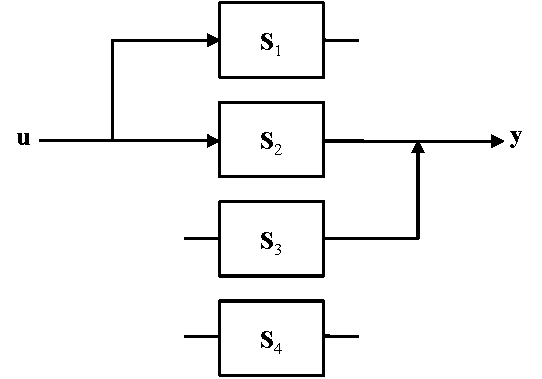
\includegraphics{pictures/partitioning.pdf}}
\end{center}
\endinput

%%% Local Variables: 
%%% mode: latex
%%% TeX-master: "notes"
%%% End:
\end{slide}
\fi

\begin{center}
	\resizebox{200pt}{!}{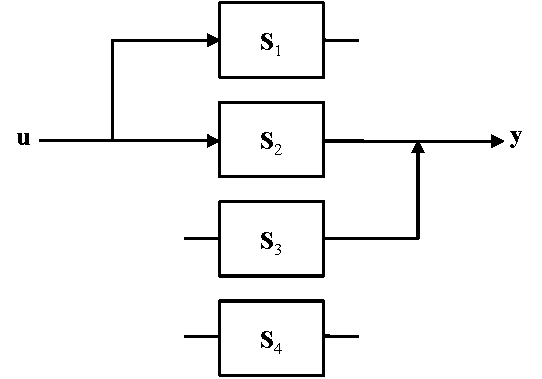
\includegraphics{pictures/partitioning.pdf}}
\end{center}
\endinput

%%% Local Variables: 
%%% mode: latex
%%% TeX-master: "notes"
%%% End:

\ifslidesonly
\begin{slide}
  \heading{Laplace transform of a vector of functions (cont)}
  If we write down the equations for the elements we get:
\begin{eqnarray}
  \frac{dv_{31}}{dt} &=& \frac{1}{C}\ i_2 \label{eq:l13e1}\\
  \frac{di_{i}}{dt} &=& \frac{1}{L}\ v_{32} \label{eq:l13e2}\\
  v_{21} &=& R\ i_1 \label{eq:l13e3}
\end{eqnarray}
The ``compatability'' and ``continuity'' equations are
\begin{eqnarray}
  u &=& i_1 + i_2 \label{eq:l13e4}\\
  v_{31} &=& v_{32} + v_{21} \label{eq:l13e5}
\end{eqnarray}

\endinput
%%% Local Variables: 
%%% mode: latex
%%% TeX-master: "notes"
%%% End: 

\end{slide}
\fi
If we write down the equations for the elements we get:
\begin{eqnarray}
  \frac{dv_{31}}{dt} &=& \frac{1}{C}\ i_2 \label{eq:l13e1}\\
  \frac{di_{i}}{dt} &=& \frac{1}{L}\ v_{32} \label{eq:l13e2}\\
  v_{21} &=& R\ i_1 \label{eq:l13e3}
\end{eqnarray}
The ``compatability'' and ``continuity'' equations are
\begin{eqnarray}
  u &=& i_1 + i_2 \label{eq:l13e4}\\
  v_{31} &=& v_{32} + v_{21} \label{eq:l13e5}
\end{eqnarray}

\endinput
%%% Local Variables: 
%%% mode: latex
%%% TeX-master: "notes"
%%% End: 


\ifslidesonly
\begin{slide}
  \heading{Example}
  Given the transformation $\mathbf{T}^{-1}\mathbf{AT}=\mathbf{\Lambda}$:
\begin{eqnarray*}
	\mathbf{A}t & = & (\mathbf{T\Lambda T}^{-1}) t \\
	\mathbf{A}^nt^n & = & (\mathbf{T\Lambda T}^{-1})(\mathbf{T\Lambda T}^{-1})\ldots(\mathbf{T\Lambda T}^{-1})t^n \\
	                & = & \mathbf{T\Lambda T}^{-1}\mathbf{T\Lambda T}^{-1}\ldots\mathbf{T\Lambda T}^{-1}t^n \\
	\mathbf{A}^nt^n & = & \mathbf{T\Lambda}\mathbf{I}\mathbf{\Lambda I}\ldots\mathbf{I\Lambda T}^{-1}t^n \\
	\               & = & \mathbf{T\Lambda}^n\mathbf{T}^{-1}t^n \\
\end{eqnarray*}
\endinput

%%% Local Variables: 
%%% mode: latex
%%% TeX-master: "notes"
%%% End:
\end{slide}
\fi
Given the transformation $\mathbf{T}^{-1}\mathbf{AT}=\mathbf{\Lambda}$:
\begin{eqnarray*}
	\mathbf{A}t & = & (\mathbf{T\Lambda T}^{-1}) t \\
	\mathbf{A}^nt^n & = & (\mathbf{T\Lambda T}^{-1})(\mathbf{T\Lambda T}^{-1})\ldots(\mathbf{T\Lambda T}^{-1})t^n \\
	                & = & \mathbf{T\Lambda T}^{-1}\mathbf{T\Lambda T}^{-1}\ldots\mathbf{T\Lambda T}^{-1}t^n \\
	\mathbf{A}^nt^n & = & \mathbf{T\Lambda}\mathbf{I}\mathbf{\Lambda I}\ldots\mathbf{I\Lambda T}^{-1}t^n \\
	\               & = & \mathbf{T\Lambda}^n\mathbf{T}^{-1}t^n \\
\end{eqnarray*}
\endinput

%%% Local Variables: 
%%% mode: latex
%%% TeX-master: "notes"
%%% End:
\ifslidesonly
  \begin{slide}
    \heading{Transform of state equations}
    The matrix function becomes:
\begin{eqnarray*}
	f(\mathbf{A}t) & = & f_0\mathbf{TIT}^{-1} + f_1\mathbf{T\Lambda T}^{-1}t + f_2\mathbf{T\Lambda}^2\mathbf{T}^{-1}t^2 + \cdots + f_n\mathbf{T\Lambda}^n\mathbf{T}^{-1}t^n + \cdots \\
	f(\mathbf{A}t) & = & \mathbf{T}\left(f_0\mathbf{I} + f_1\mathbf{\Lambda}t + f_2\mathbf{\Lambda}^2t^2 + \cdots + f_n\mathbf{\Lambda}^nt^n + \cdots \right)\mathbf{T}^{-1}\\
	               & = & \mathbf{T}f(\mathbf{\Lambda}t)\mathbf{T}^{-1}
\end{eqnarray*}
 
The term inside the brackets on the rhs is a diagonal matrix and the $i^\mathrm{th}$ diagonal element is:
\[
f_0+f_1\lambda_it + f_2\lambda_i^2t^2 + \cdots + f_n\lambda_i^nt^ + \cdots
\]
From the Taylor series this must be $f(\lambda_i t)$:
\[
f(\mathbf{A} t)=\mathbf{T} f(\mathbf{\Lambda} t) \mathbf{T}^{-1}
\]   
where $f(\mathbf{\Lambda} t)=\mathrm{diag}\left(f(\lambda_i t)\right)$.

\endinput

%%% Local Variables: 
%%% mode: latex
%%% TeX-master: "notes"
%%% End:
  \end{slide}
\fi
The matrix function becomes:
\begin{eqnarray*}
	f(\mathbf{A}t) & = & f_0\mathbf{TIT}^{-1} + f_1\mathbf{T\Lambda T}^{-1}t + f_2\mathbf{T\Lambda}^2\mathbf{T}^{-1}t^2 + \cdots + f_n\mathbf{T\Lambda}^n\mathbf{T}^{-1}t^n + \cdots \\
	f(\mathbf{A}t) & = & \mathbf{T}\left(f_0\mathbf{I} + f_1\mathbf{\Lambda}t + f_2\mathbf{\Lambda}^2t^2 + \cdots + f_n\mathbf{\Lambda}^nt^n + \cdots \right)\mathbf{T}^{-1}\\
	               & = & \mathbf{T}f(\mathbf{\Lambda}t)\mathbf{T}^{-1}
\end{eqnarray*}
 
The term inside the brackets on the rhs is a diagonal matrix and the $i^\mathrm{th}$ diagonal element is:
\[
f_0+f_1\lambda_it + f_2\lambda_i^2t^2 + \cdots + f_n\lambda_i^nt^ + \cdots
\]
From the Taylor series this must be $f(\lambda_i t)$:
\[
f(\mathbf{A} t)=\mathbf{T} f(\mathbf{\Lambda} t) \mathbf{T}^{-1}
\]   
where $f(\mathbf{\Lambda} t)=\mathrm{diag}\left(f(\lambda_i t)\right)$.

\endinput

%%% Local Variables: 
%%% mode: latex
%%% TeX-master: "notes"
%%% End:

For the system in the example the state vector is defined as
$\mathbf{x}=[v_{31}, i_1]^{T}$, the input current is $u$, and the output
variables are all the currents and voltages in the circuit
$\mathbf{y}=[v_{31}, i_1, v_{32}, v_{21}, i_2]^{T}$. The transformed
state space model is therefore that shown in
\sref{slide:slide-l2eg1}.
\begin{slide}\label{slide:slide-l2eg1}
\heading{Transformed State-Equations for Example 1 from L12}
\begin{eqnarray*} s\left[\begin{array}{c}
  V_{31} \\
  I_1
\end{array}\right]-\left[\begin{array}{c}
  v_{31}(0) \\
  i_1(0)
\end{array}\right]&=&\left[\begin{array}{cc}
  0 & -1/C \\
  1/L & -R/L
\end{array}\right]\left[\begin{array}{c}
  V_{31} \\
  I_1
\end{array}\right]+\left[\begin{array}{c}
  1/C \\
  0
\end{array}\right]\left[U\right]\\
\left[\begin{array}{c}
  V_{31} \\
  I_1 \\
  V_{32} \\
  V_{21} \\
  I_{2}
\end{array}\right]&=&\left[\begin{array}{cc}
  1 & 0 \\
  0 & 1 \\
  1 & -R \\
  0 & R \\
  0 & -1
\end{array}\right]\left[\begin{array}{c}
  V_{31} \\
  I_1
\end{array}\right]+\left[\begin{array}{c}
  0 \\
  0 \\
  0 \\
  0 \\
  1
\end{array}\right]\left[U\right].
\end{eqnarray*}
\end{slide}

\ifslidesonly
\begin{slide}
\heading{Transfer function from state space models (1)}
The vector $[v_{31}, i_{1}]^T$ is called the ``\emph{state
vector}.'' Its elements are state variables.
\endinput
%%% Local Variables: 
%%% mode: latex
%%% TeX-master: "notes"
%%% End: 

\end{slide}\fiThe vector $[v_{31}, i_{1}]^T$ is called the ``\emph{state
vector}.'' Its elements are state variables.
\endinput
%%% Local Variables: 
%%% mode: latex
%%% TeX-master: "notes"
%%% End: 

\ifslidesonly
\begin{slide}\heading{Transfer function from state space models (2)}
From previous work the error dynamics are:
\[
\dot{\mathbf{e}} = (\mathbf{A}-\mathbf{LC})\mathbf{e}
\]
Therefore the dynamics of the combined system is:
\[\left[ {\begin{array}{*{20}c}
   {\dot{\mathbf{x}}}  \\
   {\dot{\mathbf{e}}ß}  \\
\end{array}} \right] = \left[ {\begin{array}{*{20}c}
   {\left( {{\bf{A}} - {\bf{BK}}} \right)} & {{\bf{BK}}}  \\
   {\bf{0}} & {\left( {{\bf{A}} - {\bf{LC}}} \right)}  \\
\end{array}} \right]\left[ {\begin{array}{*{20}c}
   {\bf{x}}  \\
   {\bf{e}}  \\
\end{array}} \right] + \left[ {\begin{array}{*{20}c}
   {\bf{B}}  \\
   {\bf{0}}  \\
\end{array}} \right]r
\]
\endinput

%%% Local Variables: 
%%% mode: latex
%%% TeX-master: "notes"
%%% End:
\end{slide}\fiFrom previous work the error dynamics are:
\[
\dot{\mathbf{e}} = (\mathbf{A}-\mathbf{LC})\mathbf{e}
\]
Therefore the dynamics of the combined system is:
\[\left[ {\begin{array}{*{20}c}
   {\dot{\mathbf{x}}}  \\
   {\dot{\mathbf{e}}ß}  \\
\end{array}} \right] = \left[ {\begin{array}{*{20}c}
   {\left( {{\bf{A}} - {\bf{BK}}} \right)} & {{\bf{BK}}}  \\
   {\bf{0}} & {\left( {{\bf{A}} - {\bf{LC}}} \right)}  \\
\end{array}} \right]\left[ {\begin{array}{*{20}c}
   {\bf{x}}  \\
   {\bf{e}}  \\
\end{array}} \right] + \left[ {\begin{array}{*{20}c}
   {\bf{B}}  \\
   {\bf{0}}  \\
\end{array}} \right]r
\]
\endinput

%%% Local Variables: 
%%% mode: latex
%%% TeX-master: "notes"
%%% End:
\ifslidesonly
\begin{slide}\heading{Transfer function from state space models (3)}
When the initial conditions of the state-variables are all zero,
this reduces to the transfer matrix model
\begin{equation}\label{eqn:transfer-function}
  \mathbf{Y}=\left[\mathbf{C}\left[s\mathbf{I}-\mathbf{A}\right]^{-1}\mathbf{B}+\mathbf{D}\right]\mathbf{U}
\end{equation}

\endinput

%%% Local Variables: 
%%% mode: latex
%%% TeX-master: "notes"
%%% End: 

\end{slide}\fiWhen the initial conditions of the state-variables are all zero,
this reduces to the transfer matrix model
\begin{equation}\label{eqn:transfer-function}
  \mathbf{Y}=\left[\mathbf{C}\left[s\mathbf{I}-\mathbf{A}\right]^{-1}\mathbf{B}+\mathbf{D}\right]\mathbf{U}
\end{equation}

\endinput

%%% Local Variables: 
%%% mode: latex
%%% TeX-master: "notes"
%%% End: 

\ifslidesonly
\begin{slide}\heading{Transfer function from state space models (4)}
When the observer canonical form is not used, then the design of the observer is more difficult. Ackermann's formula can be adapted as follows:
% MathType!MTEF!2!1!+-
% faaagaart1ev2aaaKnaaaaWenf2ys9wBH5garuavP1wzZbqedmvETj
% 2BSbqefm0B1jxALjharqqtubsr4rNCHbGeaGqiVu0Je9sqqrpepC0x
% bbL8FesqqrFfpeea0xe9Lq-Jc9vqaqpepm0xbba9pwe9Q8fs0-yqaq
% pepae9pg0FirpepeKkFr0xfr-xfr-xb9Gqpi0dc9adbaqaaeGaciGa
% aiaabeqaamaabaabaaGcbaGaaCitamaaCaaaleqabaGaamivaaaaki
% abg2da9maadmaabaqbamqabeabaaaabaGaaGimaaqaaiablAcilbqa
% aiaaicdaaeaacaaIXaaaaaGaay5waiaaw2faaiaad+eadaahaaWcbe
% qaaiabgkHiTiaaigdaaaGccqaHXoqydaWgaaWcbaGaam4yaaqabaGc
% caGGOaGaaCyqamaaCaaaleqabaGaamivaaaakiaacMcaaaa!3EF6!
\[
{\bf{L}}^T  = \left[ {\begin{array}{*{20}c}
   0 &  \ldots  & 0 & 1  \\
\end{array}} \right]\mathcal{O}^{ - 1} \alpha _e ({\bf{A}}^T )
\]
$\mathcal{O}$ is the observability matrix:
\[
\mathcal{O}=[\mathbf{C}^T\vdots\mathbf{A}^T\mathbf{C}^T\vdots\cdots\vdots(\mathbf{A}^T)^{n-1}\mathbf{C}^T]
\]
and if $\alpha_e(s)=s^n + \alpha_1s^{n-1}+\cdots+\alpha_n$ then \[\alpha_e(\mathbf{A}^T)=(\mathbf{A}^T)^n + \alpha_1(\mathbf{A}^T)^{n-1}+\cdots+\mathbf{I}\alpha_n.\]
 

Notice that if the system is unobservable, then the matrix inverse $\mathcal{O}^{-1}$ does not exist and we cannot design an observer for this system.


 
 

\endinput

%%% Local Variables: 
%%% mode: latex
%%% TeX-master: "notes"
%%% End:\end{slide}\fiWhen the observer canonical form is not used, then the design of the observer is more difficult. Ackermann's formula can be adapted as follows:
% MathType!MTEF!2!1!+-
% faaagaart1ev2aaaKnaaaaWenf2ys9wBH5garuavP1wzZbqedmvETj
% 2BSbqefm0B1jxALjharqqtubsr4rNCHbGeaGqiVu0Je9sqqrpepC0x
% bbL8FesqqrFfpeea0xe9Lq-Jc9vqaqpepm0xbba9pwe9Q8fs0-yqaq
% pepae9pg0FirpepeKkFr0xfr-xfr-xb9Gqpi0dc9adbaqaaeGaciGa
% aiaabeqaamaabaabaaGcbaGaaCitamaaCaaaleqabaGaamivaaaaki
% abg2da9maadmaabaqbamqabeabaaaabaGaaGimaaqaaiablAcilbqa
% aiaaicdaaeaacaaIXaaaaaGaay5waiaaw2faaiaad+eadaahaaWcbe
% qaaiabgkHiTiaaigdaaaGccqaHXoqydaWgaaWcbaGaam4yaaqabaGc
% caGGOaGaaCyqamaaCaaaleqabaGaamivaaaakiaacMcaaaa!3EF6!
\[
{\bf{L}}^T  = \left[ {\begin{array}{*{20}c}
   0 &  \ldots  & 0 & 1  \\
\end{array}} \right]\mathcal{O}^{ - 1} \alpha _e ({\bf{A}}^T )
\]
$\mathcal{O}$ is the observability matrix:
\[
\mathcal{O}=[\mathbf{C}^T\vdots\mathbf{A}^T\mathbf{C}^T\vdots\cdots\vdots(\mathbf{A}^T)^{n-1}\mathbf{C}^T]
\]
and if $\alpha_e(s)=s^n + \alpha_1s^{n-1}+\cdots+\alpha_n$ then \[\alpha_e(\mathbf{A}^T)=(\mathbf{A}^T)^n + \alpha_1(\mathbf{A}^T)^{n-1}+\cdots+\mathbf{I}\alpha_n.\]
 

Notice that if the system is unobservable, then the matrix inverse $\mathcal{O}^{-1}$ does not exist and we cannot design an observer for this system.


 
 

\endinput

%%% Local Variables: 
%%% mode: latex
%%% TeX-master: "notes"
%%% End:
\ifslidesonly
\begin{slide}\heading{The Resolvant Matrix}
\begin{itemize}
	\item Rule of thumb: observer poles can be faster than the controller poles (i.e. further from the origin) by a factor of 2 to 6. This makes the effect of the observer dynamics short-term and the overall response is dominated by the controller poles.
	\item If noise/disturbance is present this has an effect on the choice:
	\begin{description}
		\item[Process noise $w$:] $d\mathbf{x}/dt=\mathbf{Ax}+\mathbf{B}u+\mathbf{B}_1 w$
		\item[Sensor noise $v$:]  $y = \mathbf{C}x+v$
		\item[Observer:] $d\hat{\mathbf{x}}=\mathbf{A}\hat{\mathbf{x}}+\mathbf{B}u+\mathbf{L}(y-\mathbf{C}\hat{\mathbf{x}})$
		\item[Error $\mathbf{e}=\mathbf{x}-\hat{\mathbf{x}}$:] $d\mathbf{e}/dt=(\mathbf{A}-\mathbf{LC})\mathbf{e}+\mathbf{B}_1 w - \mathbf{L}v.$
	\end{description}
\end{itemize}

\endinput

%%% Local Variables: 
%%% mode: latex
%%% TeX-master: "notes"
%%% End:\end{slide}\fi\begin{itemize}
	\item Rule of thumb: observer poles can be faster than the controller poles (i.e. further from the origin) by a factor of 2 to 6. This makes the effect of the observer dynamics short-term and the overall response is dominated by the controller poles.
	\item If noise/disturbance is present this has an effect on the choice:
	\begin{description}
		\item[Process noise $w$:] $d\mathbf{x}/dt=\mathbf{Ax}+\mathbf{B}u+\mathbf{B}_1 w$
		\item[Sensor noise $v$:]  $y = \mathbf{C}x+v$
		\item[Observer:] $d\hat{\mathbf{x}}=\mathbf{A}\hat{\mathbf{x}}+\mathbf{B}u+\mathbf{L}(y-\mathbf{C}\hat{\mathbf{x}})$
		\item[Error $\mathbf{e}=\mathbf{x}-\hat{\mathbf{x}}$:] $d\mathbf{e}/dt=(\mathbf{A}-\mathbf{LC})\mathbf{e}+\mathbf{B}_1 w - \mathbf{L}v.$
	\end{description}
\end{itemize}

\endinput

%%% Local Variables: 
%%% mode: latex
%%% TeX-master: "notes"
%%% End:

For the system in the example, the resolvent matrix is developed
in \sref{slide:l2eg2}.
\begin{slide}\label{slide:l2eg2}
\heading{Resolvent matrix for the example}
\begin{eqnarray*}
\mathbf{A}&=&\left[\begin{array}{cc}
  0 & -1/C \\
  1/L & -R/L
\end{array}\right] \\
s\mathbf{I}-\mathbf{A}&=&\left[
\begin{array}{cc}
  s & 0 \\
  0 & s
\end{array}
\right] - \left[
\begin{array}{cc}
  0 & -1/C \\
  1/L & -R/L
\end{array}
\right] = \left[
\begin{array}{cc}
  s & +1/C \\
  -1/L & s+R/L
\end{array}\right] \\
\left[s\mathbf{I}-\mathbf{A}\right]^{-1}&=&\frac{
\left[\begin{array}{cc}
  s+R/L & -1/C \\
  +1/L & s
\end{array} \right]
}{s(s+R/L)+1/(LC)}=\frac{\left[\begin{array}{cc}
  s+R/L & -1/C \\
  +1/L & s
\end{array} \right]}{s^2 + (R/L)s + 1/(LC) }
\end{eqnarray*}
\end{slide}

When $\left[s\mathbf{I}-\mathbf{A}\right]^{-1}$ has been obtained,
then the system transfer function is easily obtained through
$\mathbf{C}\left[s\mathbf{I}-\mathbf{A}\right]^{-1}\mathbf{B}+\mathbf{D}$.
For the system in the example, when all outputs are measured, the
system transfer matrix is that shown in \sref{slide:l2eg3}.

\begin{slide}\label{slide:l2eg3}
\heading{Transfer matrix for example}
\begin{eqnarray*}
\left[\begin{array}{cc}
  1 & 0 \\
  0 & 1 \\
  1 & -R \\
  0 & R \\
  0 & -1
\end{array}\right]
\left\{\frac{\left[
\begin{array}{cc}
  s+R/L & -1/C \\
 +1/L & s
\end{array}\right]}{s^2 + (R/L)s +1/(LC)}\right\}
\left[\begin{array}{c}
  1/C \\
  0
\end{array}\right]
 &+& \left[\begin{array}{c}
  0 \\
  0 \\
  0 \\
  0 \\
  1
\end{array} \right]\\
= \left[\begin{array}{cc}
  1 & 0 \\
  0 & 1 \\
  1 & -R \\
  0 & R \\
  0 & -1
\end{array}\right]
\left\{\frac{\left[
\begin{array}{c}
  (1/C)s+R/(LC)  \\
 +1/(LC)
\end{array}\right]}{s^2 + (R/L)s +1/(LC)}\right\}
 &+& \left[\begin{array}{c}
  0 \\
  0 \\
  0 \\
  0 \\
  1
\end{array} \right]\\
\end{eqnarray*}
\end{slide}
\begin{slide}
\heading{Transfer matrix for example (completed)}
\begin{eqnarray*} &=& \frac{1}{s^2 + (R/L)s
+1/(LC)}\left[\begin{array}{c}
  (1/C)s+R/(LC) \\
  1/(LC) \\
  (1/C)s \\
  R/(LC) \\
  -1/(LC)
\end{array}\right] + \left[\begin{array}{c}
  0 \\
  0 \\
  0 \\
  0 \\
  1
\end{array} \right]\\
&=& \left[\begin{array}{c}
  \frac{(1/C)s+R/(LC)}{s^2 + (R/L)s
+1/(LC)} \\
  \frac{1/(LC)}{s^2 + (R/L)s
+1/(LC)} \\
  \frac{(1/C)s}{s^2 + (R/L)s
+1/(LC)} \\
  \frac{R/(LC)}{s^2 + (R/L)s
+1/(LC)} \\
  -\frac{1/(LC)}{s^2 + (R/L)s
+1/(LC)}+1
\end{array}\right]
\end{eqnarray*}
\end{slide}

In matrix form, when combined with the input and output transforms we
have the situtaion illustrated in \sref{slide:l2final}.
Each transfer function relates the corresponding output transform
to the input transform. For example
\[V_{31}= \frac{(1/C)s+R/(LC)}{s^2 + (R/L)s
+1/(LC)}\ U.\]

\begin{slide}
  \label{slide:l2final}
  \heading{Transform Equations for Example}
\begin{eqnarray*}
\mathbf{Y}(s)&=&\left[\mathbf{C}\left[s\mathbf{I}-\mathbf{A}\right]^{-1}\mathbf{B}+\mathbf{D}\right]\mathbf{U}(s)\\
\mathbf{Y}(s) &=& \mathbf{G}(s)\mathbf{U}(s)\\
\left[\begin{array}{c}
  V_{31}(s) \\
  I_1(s) \\
  V_{32}(s) \\
  V_{21}(s) \\
  I_{2}(s)
\end{array}\right] &=& \left[\begin{array}{c}
  \frac{(1/C)s+R/(LC)}{s^2 + (R/L)s
+1/(LC)} \\
  \frac{1/(LC)}{s^2 + (R/L)s
+1/(LC)} \\
  \frac{(1/C)s}{s^2 + (R/L)s
+1/(LC)} \\
  \frac{R/(LC)}{s^2 + (R/L)s
+1/(LC)} \\
  -\frac{1/(LC)}{s^2 + (R/L)s
+1/(LC)}+1
\end{array}\right]\mathbf{U}(s).
\end{eqnarray*}
\end{slide}
Note that the denominator is the same for each transfer function,
and that the order of the numerator is less than the denominator
except for one case, for which
\begin{eqnarray*}
I_2 & = & \left(-\frac{1/(LC)}{s^2 + (R/L)s +1/(LC)}+1\right)U\\
    & = & \frac{-1/{LC}+s^2 + (R/L)s +1/(LC)}{s^2 + (R/L)s
    +1/(LC)}\ U
    \\
    & = &\frac{s^2 + (R/L)s}{s^2 + (R/L)s
    +1/(LC)}\ U
\end{eqnarray*}
Replacing $s$ by $\frac{d}{dt}$ gives the corresponding
differential equations relating the dependant variable to the
input.

\begin{slide}
	\heading{Converting SS to TF in Matlab}
	Continuing example from previous lecture
	\begin{verbatim}
		circ_tf = tf(circ_ss)
	\end{verbatim}
	Returns a vector of transfer functions.
\end{slide}

\subsection*{Some Important Properties}

\subsubsection*{System poles}

Clearly the denominator of the transfer function is generated by the matrix inverse which produces the term:
$$\det[s\mathbf{I}-\mathbf{A}]$$
 
This evaluates to the denominator polynomial and the poles of the system are the roots of the system's characteristic equation:
$$\det[s\mathbf{I}-\mathbf{A}] = 0.$$
\ifslidesonly
\begin{slide}
	\heading{System Poles}
	The system poles are solutions to the system's characteristic equation
	$$\det[s\mathbf{I}-\mathbf{A}] = 0.$$
\end{slide}
\fi


\subsubsection*{System zeros}

What is the corresponding numerator polynomial of the transfer function, whose roots give the zeros of the system?
The zeros are those values of $s$ for which the output is zero when the input and states are not zero. Thus:
\begin{eqnarray*}
(s\mathbf{I}-\mathbf{A})\mathbf{x}-\mathbf{B}U & = & \mathbf{0} \\
\mathbf{Cx}+dU = Y & = & 0
\end{eqnarray*}
The last example had a system TF with no zeros. In this case it is easy to construct the equivalent classical controller. We had the feedback law:
\[
u=r-5x_1-156x_2
\]

Now $y=7x_2$ and $\dot{x}_2=x_1$ therefore $X_2(s)=Y(s)/7$ and $X_1(s)=sX_2(s)=sY(s)/7$. Therefore
\begin{eqnarray*}
	U(s) & = & R(s)-rX_1(s)-156X_2(s) \\
	& = & R(s) - \frac{1}{7}(5s+156)Y(s)
\end{eqnarray*}

\endinput

%%% Local Variables: 
%%% mode: latex
%%% TeX-master: "notes"
%%% End:
\ifslidesonly
\begin{slide}
	\heading{System Zeros (1)}
	Zeros are those values of $s$ for which the system output is zero when the input and states are not zero
	\begin{eqnarray*}
		(s\mathbf{I}-\mathbf{A})\mathbf{x}-\mathbf{B}U & = & \mathbf{0} \\
		\mathbf{Cx}+dU = Y & = & 0
	\end{eqnarray*}
	The last example had a system TF with no zeros. In this case it is easy to construct the equivalent classical controller. We had the feedback law:
\[
u=r-5x_1-156x_2
\]

Now $y=7x_2$ and $\dot{x}_2=x_1$ therefore $X_2(s)=Y(s)/7$ and $X_1(s)=sX_2(s)=sY(s)/7$. Therefore
\begin{eqnarray*}
	U(s) & = & R(s)-rX_1(s)-156X_2(s) \\
	& = & R(s) - \frac{1}{7}(5s+156)Y(s)
\end{eqnarray*}

\endinput

%%% Local Variables: 
%%% mode: latex
%%% TeX-master: "notes"
%%% End:
\end{slide}
\fi
 
\[
s{\bf{\hat X}}(s) =  {\bf{A\hat X}}(s) + {\bf{B}}U(s) + {\bf{L}}\left( {Y(s) - {\bf{C\hat X}}}(s) \right)
\]
then,
\[
\left( {s{\bf{I}} - {\bf{A}} + {\bf{LC}}} \right){\bf{\hat X}}(s) = {\bf{B}}U(s) + {\bf{L}}Y(s) 
\]
or,
\[
{\bf{\hat X}}(s) = {\bf{M}}^{ - 1} {\bf{B}}U(s) + {\bf{M}}^{ - 1} {\bf{L}}Y(s)
\]


\endinput

%%% Local Variables: 
%%% mode: latex
%%% TeX-master: "notes"
%%% End:
\ifslidesonly
\begin{slide}
	\heading{System Zeros (2)}
	\[
s{\bf{\hat X}}(s) =  {\bf{A\hat X}}(s) + {\bf{B}}U(s) + {\bf{L}}\left( {Y(s) - {\bf{C\hat X}}}(s) \right)
\]
then,
\[
\left( {s{\bf{I}} - {\bf{A}} + {\bf{LC}}} \right){\bf{\hat X}}(s) = {\bf{B}}U(s) + {\bf{L}}Y(s) 
\]
or,
\[
{\bf{\hat X}}(s) = {\bf{M}}^{ - 1} {\bf{B}}U(s) + {\bf{M}}^{ - 1} {\bf{L}}Y(s)
\]


\endinput

%%% Local Variables: 
%%% mode: latex
%%% TeX-master: "notes"
%%% End:
\end{slide}
\fi



Now
\[
U(s) =  - {\bf{K\hat X}}(s) 
\]
so
\[
U (s) =   - {\bf{K}}\left( {{\bf{M}}^{ - 1} {\bf{B}}U(s) + {\bf{M}}^{ - 1} {\bf{L}}Y(s)} \right) 
\]
\[
 \left( {1 + {\bf{KM}}^{ - 1} {\bf{B}}} \right)U(s) =  - {\bf{KM}}^{ - 1} {\bf{L}}Y(s)
\]

\[ 
H\left( s \right) =  - \frac{U(s)}{Y(sßß)} = \frac{{{\bf{KM}}^{ - 1} {\bf{L}}}}{{1 + {\bf{KM}}^{ - 1} {\bf{B}}}} 
\]




\endinput

%%% Local Variables: 
%%% mode: latex
%%% TeX-master: "notes"
%%% End:
\ifslidesonly
\begin{slide}
	\heading{System Zeros (3)}
	Now
\[
U(s) =  - {\bf{K\hat X}}(s) 
\]
so
\[
U (s) =   - {\bf{K}}\left( {{\bf{M}}^{ - 1} {\bf{B}}U(s) + {\bf{M}}^{ - 1} {\bf{L}}Y(s)} \right) 
\]
\[
 \left( {1 + {\bf{KM}}^{ - 1} {\bf{B}}} \right)U(s) =  - {\bf{KM}}^{ - 1} {\bf{L}}Y(s)
\]

\[ 
H\left( s \right) =  - \frac{U(s)}{Y(sßß)} = \frac{{{\bf{KM}}^{ - 1} {\bf{L}}}}{{1 + {\bf{KM}}^{ - 1} {\bf{B}}}} 
\]




\endinput

%%% Local Variables: 
%%% mode: latex
%%% TeX-master: "notes"
%%% End:
\end{slide}
\fi

\begin{slide}
	\heading{Determine Poles and Zeros in Matlab}
	\begin{verbatim}
		circ_zpk = zpk(circ_ss)
	\end{verbatim}
\end{slide}

%----------------------------------------------------------------
% The end of slides
% ----------------------------------------------------------------
\endinput

%%% Local Variables: 
%%% mode: latex
%%% TeX-master: "#"
%%% End: 
